
\chapter{A Review of Solving Partial Differential Equations (PDEs)}
\section{About PDEs}

Partial differential equations (PDEs) are used to model many real world phenomena such as wave propagation, fluid flow, heat flow and distribution, etc. A linear 2nd-Order PDE of the general form is:\\
$Au_{xx} + 2Bu_{xy} + Cu_{yy} + Du_{x} + Eu_{y} + Fu + G = 0$\\
where the coefficients A, B, C etc.  may depend upon x and y. 

If $(A^2+ B^2+C^2) >0$ over a region of the x-y plane, the PDE is second-order in that region. PDEs can be classified into elliptic, parabolic and hyperbolic equations. The classification is based in the discriminant $B^2 – 4AC$ as shown in Table 3.1. Parabolic equations, with the thermal conductivity equation as the most characteristic example, involve time dependency and describe diffusion. Hyperbolic equations, with the wave equation as the most standard example, are time dependent and describe dissemination phenomena. Unlike the previous, elliptic equations describe the static behavior of a magnitude in a particular area without time dependency. The most characteristic elliptical equation is the Laplace equation. Parabolic and hyperbolic equations are usually defined as initial value problems and elliptic equations as boundary value problems.

\begin{table}[H]
    \begin{center}
        \begin{tabular}{| l | l |}
        \hline
        Discriminant   & Type 	\\ \hline
        $B^2 – 4AC < 0$   & Elliptic (e.g. Laplace Eq.) 	\\ \hline
        $B^2  – 4AC = 0$  &	Parabolic (e.g. Heat Eq.)        \\ \hline
        $B^2 – 4AC > 0$  & Hyperbolic (e.g. Wave Eq.) 	\\ \hline       
        \end{tabular}
    \end{center}
    \caption{Classification of PDEs}
    \label{table:trainingset}
\end{table}

Most frequently, PDEs are solved using Finite Difference (FD), Finite Element Methods (FEM) and Finite Volume (FV) methods. The Finite Difference technique is implemented and mathematically analyzed more easily than the other techniques, since they formulated for structured meshes/grids. The least popular is the Finite Volume approximation because it is only two decades scientists are working on them but they are highly known further for high accuracy results in both structured and unstructured meshes.

\subsection{Finite Difference Methods for Solving Elliptic PDEs}
The first step concerns the discretization of the PDE domain into a grid of evenly spaced points (nodes) and the restriction of the PDE equation on these nodes. The second step involves the discretization of the partial derivatives and possibly its boundary conditions for every grid node. For the 2-D simple PDE problem\\
$u_{xx}+u_{yy}+ u=f$   in $\Omega$,   $u=g$ on   $\partial  \Omega $ \\
and if the (1-21) stencil for the discretization of the second derivative is used, then the continuous equation becomes the following system of linear equations:

\[ \frac{\partial^2 u}{\partial^2 x} + \frac{\partial^2 u}{\partial^2 y}
   = \ \frac{\ u_{i-1,j} -2u_{i,j} + u_{i+1,j} }{\\\Delta x^2}\ + \ \frac{\ u_{i,j-1} -2u_{i,j} + u_{i,j+1} }{\\\Delta y^2}\]
      
The scheme used in this example is Finite Difference scheme, since it considers a central node and four neighbors. If the accuracy of the results is of major importance, Finite Difference schemes with accuracy higher than second order can be used. These equations involve more than four neighbor nodes, e.g., the nine point scheme. The extension of this method in 3-D can be done easily, increasing the number of the nodes involved in the equation. In this case the equations involve seven and twenty-seven neighbor nodes for second or higher order accuracy, respectively. 

The final step concerns the solution of the resulting linear system. The linear algebra methods for the solution  are divided in two basic categories, Iterative (Jacobi, Gauss-Seidel, SOR, Multigrid etc) and direct methods (Gauss, Cholesky, Thomas, FFT etc).

\subsection{Finite Difference Methods for Solving Parabolic PDE's}
The first step, as before concerns the discretization of the domain into grid of evenly spaced points (nodes). The second step involves the expression of the derivatives in terms of Finite Difference Approximations of $O(h^2)$ and $O(Δt)$ [or $O(Δt^2)$ order ] :

$\frac{\partial^2 T}{\partial^2 x} , \frac{\partial^2 T}{\partial^2 y} , \frac{\partial T}{\partial t}  \Longrightarrow Finite   Differences $

As a final step, remains the choice of $h = Δx = Δy$, and $Δt$ and use of the initial and boundary conditions to solve the problem by systematically moving ahead in time. For the time derivative referred above, explicit (Euler, Leapfrog, Runge-Kutta) and implicit (Crank-Nicolson Method, ADI methods, etc.) schemes are used. Explicit methods express all future values $(t + Δt)$ in terms of current $(t)$ and previous $(t - Δt)$ information, which are known. Implicit methods derive future values $(t + Δt)$ by solving appropriate equations in terms of current $(t)$ and sometimes previous $(t - Δt)$ information.

\section{Stencil Computation}
As shown above, Finite Difference methods are mainly used as the second step of the PDE solution. These methods perform nearest neighbor computations called stencils. In stencil computations, each point of the grid is updated depending on a subset of its neighbors. In this way, the coefficients of the PDE are represented. Excessive work is done in this field aiming to achieve efficiency, optimization and high performance on GPUs. 

Brandvik and Pullan [5] present a generalized software framework named SBLOCK for applications that use stencil computations to solve PDEs. They used the 3D heat diffusion equation as a model problem to demonstrate their results. A second order center Finite Difference approximation scheme is used for the derivatives and the Jacobi iterative method is used for the solution of the derived system of the linear equation.  According to the authors their main contribution is the combination of the automatic source code generation with a run-time library. The run-time library provides an API that is used by the application for different functions and is divided in host library and device library. The application interacts with the run-time library either through the host library or by making calls directly to the device library. This host-device abstraction is useful since only a new device library has to be written to support a new type of processor, the host library always remains the same. One of the problems is the performance bottleneck caused by the transfer of the data across the PCI-Express bus. This can be solved in different ways, depending on the problem. If the boundary conditions can be expressed in the form of a SpMV, the application can use SBLOCK’s SpMV library directly. Therefore no data will be transferred across the PCI-E bus unless it needs information from another processor. If the boundary conditions are expressed differently the application may request a pointer to the array directly from the device library, and implement its own functions in NVIDIA’s CUDA language to operate on this array. For the second component, the source code generation, it is important to highlight that with this approach firstly they achieved to enable multiple platforms using only a single, high-level definition of the computations performed by the solver. Secondly, because of the abstract view of the kernel implementation that the developer has, SBLOCK can use any optimization strategy offering code readability. The optimization strategies which were used by the framework were about achieving high performance using domain decompositioning and multiple threads. Moreover to maximize the amount of reuse of data in the on-chip memories, they used the "cyclical queue" strategy [4]. The framework runs in both multiprocessors and GPUs. For their experiments they used: Intel Core i7 920 (Nehalem), AMD Phenom II X4 940 and NVIDIA GTX 280. The kernels of the algorithm are split into two categories: stencil kernels and non-stencil kernels. After studying the performance and the power efficiency of different important stencils, in both single and double precision, they came to the conclusion that good performance has been demonstrated for a range of stencil kernels with different stencil sizes and arithmetic intensities. They also showed that there is a good scaling across a large GPU cluster (good results up to 16 GPUs and scaling up to 64 GPUs).

Paulius in [6] describe a GPU parallelization of the 3D finite difference computation using CUDA. The main object of this paper is how the data access redundancy evaluates implementation efficiency for both stencil-only computation and discretization of the wave equation. In the implementation the goal was to reduce redundancy (the ratio between number of elements accessed and number of elements processed) by performing calculation from shared memory. In 2D computation the 2D tile was loaded in shared memory so as the output tile to be computed. In this paper they presented an extension to 3D with two approaches, two pass and single pass. The approach of the two pass traverses the input volume twice. The first pass concerns the computation of the 2D stencil values while during the second pass, the partial results from the first pass are combined. With this approach they referred that they had an important improvement in redundancy over the naive approach which computes an order k-stencil by re-fetching all input elements for every output value, and it becomes better with the single-pass approach. Experiments were performed on stencil-only computations and on finite difference of the wave equation. About the stencil-only computation all configurations were processed using 16 x 16 thread blocks operating 16 x 16 output tiles. The experiments concerned different volume dimensions in relation to order in space, where throughput evaluated as a metric. These experiments showed that for fixed volume dimensions, throughput decrease with increased orders, is largely due to higher read redundancy, with additional arithmetic being another contributing factor. For the 3-D finite difference of the wave equation, two kernels were implemented. About the first kernel they utilized 16 x 16 thread blocks and output tiles with redundancy at order of 5. For the second kernel they utilized 32 x 16 thread blocks, 32 x 32 output tiles and the redundancy was 4.5. GPU performance was roughly an order of magnitude higher than a single 4-core Harpertown Xeon, running an optimized implementation of the same computation. It was also demonstrated a multi-GPU implementation of the wave-equation finite difference. Performance results (using 16 x 16 tiles and thread blocks arranged as 16 x 16 threads) are shown for up to 4 GPUs. It was showed an almost linear speed-up in two and four GPUs except one case(544 × 544 × 400 does not scale linearly with 4 GPUs due to the fact that each GPU computes only 100 slices which takes significantly less time than corresponding communication). They indicated that communication overhead is hidden as long as the number of slices per GPU is 200 or greater.

Foster [7] in his paper proposed three main optimizations for solving 2D parabolic PDEs using difference equations. The approach of the red-black array was used from the representation of the grid. As first optimization, they focused on the separation of the unified red-black array into a single red- array and a single black one. The division was performed on the CPU and the separated arrays were passed to the CUDA kernel. In this way they avoided divergence since the entire warp handled either red or black points. With the second optimization strategy they aimed to reduce the number of sequential memory accesses. For updating N points in the grid, it was required 5 sequential memory accesses. To eliminate this extra latency, they reduced the amount of work per thread block. The final optimization concerned the shared memory. Because of the utilization of data, they reduced redundant memory reads through shared memory storing which was faster than accessing RAM. The computer used for testing was Intel Core i7 920 at 2.67 GHz. The two graphics cards used for GPU computing were an NVIDIA Tesla and an EVGA GeForce 480. The four versions of the kernel tested were: CPU, GPU with no optimization, GPU-RB for the first optimization and GPU-RBS for the remaining two optimizations. Throughput was used as a metric with single floating point precision. First, the throughput of the CPU implementation declined quickly in all tests from 500 to about 1500 points per dimension and gradually tapered off more as the data set sizes continued to increase. Over the same range of 500 to 1500 points per side, the throughput of the GPU versions greatly increased in relation to the number of threads and the dimension of the problem. For both cards, the first strategy, with the division of the unified array, showed an important speed-up over the basic GPU implementation, while the GPU-RB version yielded speeds of around 50\%. Finally they underlined that how advantageous these strategies are, depends on the GPU architecture and GPU hardware.

Schäfer and Fey [9] presented a number of different approaches to conduct stencil computations on GPGPUs, based on a range of micro benchmarks. They choose the Jacobi iteration as a standard benchmark because it has a low FLOP per byte ratio and is the most common method. Their research is embedded into LibGeoDecomp (a generic library which can automatically parallelize user supplied stencil codes). According to this paper the performance of a stencil code is a result of a lot of things which have to be considered and they dedicated a section writing down how to achieve the GPGPU's maximum memory bandwidth, hide the several hundred cycles of memory latency and saturate the arithmetic pipelines. In each sequential Jacobi iteration, each update calculates a weighted average of the old cell with its neighbors in the six cardinal directions. The general approach was to break down the total volume into smaller chunks. Each chunk was assigned to a CUDA thread block. How the cells of a chunk are distributed among the threads of a thread block depends on the algorithm. The authors developed 3 approaches: the “naïve algorithm”, the “cached plane sweep” and the “pipelined wavefront”. In the first algorithm all seven values for single cell update are loaded directly from memory. Because of the cost of calculations which have to be carried with this algorithm they suggested an improvement related to the number of threads that update cells. In the “cached plane sweep” algorithm all threads of a block were put on a 2D plane and this plane is swept through the chunk. They paid attention on optimizations related to L1 cache reuse, so as the accesses to neighbor values in the same plane to be mostly served from L1 cache and they stored cells, in the direction of the moving plane, in registers. For the last algorithm, the “pipelined wavefront”, they take advantage of the von Neumann neighborhood’s property, that neighboring cells outside of the plane’s direction of travel have to be read only from one layer. In this way they managed to reduce planes to two. Their testbed consists of an NVIDIA GeForce GTX 480 consumer GPGPU and a Tesla C2050. All algorithms were tested with a block size of 32 x 16 x 1 threads because they found out that was the best geometry for their experiments. The “naïve” as well as the “cached plane sweep” algorithm updated blocks of 32 x 16 x 8 cells, while the “pipelined wavefront” algorithm turned out to run faster when updating 32x32x64 cells. They concluded that the “pipelined wavefront” is the fastest algorithm on the Tesla card but only for a specific size of models because shared memory is limited and as future work, performance could be improved.  

Playne and Hawick [10] in their paper presented two methods, for implementing finite difference field-equation simulations on multiple GPUs. The main issue is the reduction of communication of cell halos and the overlap communications with computations. They noticed that even if finite difference methods are used more often, first-order Euler time integration method or Runge-Kutta method are easiest. First, they deal with the determination of the size of the equation memory halo and how the equation can be split across multiple GPUs. More communication between cells in each step is required for equations with a large memory halo. The field equation used as example was the Cahn-Hilliard equation. They used the best implementation for this equation and they tried to improve this simulation by spreading the computation across two GPUs. In their paper they describe in details the basic design of the best implementation. In short texture memory is used for reading the value of the cells and the surrounding neighbors from memory. This improved significantly the performance of the simulation. For the field decomposition, the field was divided in two halves and one half is loaded into memory on each GPU and with two sets of bordering cells from the other half. The width of this model depends on the memory halo of the model. The field should be split in the highest dimension so as the cells in the borders to be in sequential addresses. The first method they present is the synchronous memory copy. For this implementation they used the pThreads library to manage the multi-threading on the CPU. The main problem was that while the CPU threads exchanged data, the each GPU stopped and sit idle. For this reason they implemented the second method, the asynchronous one. CUDA supports asynchronous host-device memory access and execution for GPUs. They used streams to split device execution so as to can take place at the same time with memory copies. This is very useful for a GPU idle time reduction. The basic idea behind this implementation was to use asynchronous copies to exchange the border cell values between the two threads while the GPU is still computing the simulation for the rest of the field. One problem worth mentioning that they faced, was that for the GPU to copy data from the device memory to the host, the host memory must be allocated by CUDA to ensure that it is page locked. This problem resolved successfully using a flag that tells the compiler to make the memory available to all CUDA contexts rather than only the one used to declare it. The GPUs used for the simulations is one NVIDIA GeForce GTX 295 which contains two GPUs. In most experiments the asynchronous memory copy implementation was shown that provide the best performance. As the field length and memory halo increasing in size the performance keep becoming better. A certainly unexpected effect was the loss in performance seen when the field lengths are not powers of two. As a conclusion, they underlined that the correct use of asynchronous memory communication can provide almost linear speed-up over a single-GPU implementation for larger system sizes.


\section{Solvers for PDEs}
After discretization, elliptic equations lead to algebraic equations. Most previous works use implicit schemes to discretize the PDEs that lead to solving a sparse linear system. Many numerical methods, such as Jacobi, Gauss–Seidel, conjugate gradient, and multigrid, have been applied. Explicit methods are more expensive but as the computing power is growing, there are a lot of works which use an explicit approach and a responding PDE solver.

Daniel Egloff  [11] [25] uses the parabolic convection diffusion equation $\frac{du}{dt} = L_(t )*u(t,x)$   where, in case of a single risk factor, Lt is the differential operator, to present a tridiagonal solver on GPUs using cyclic reduction .The purpose of this is to improve  the performance of  finite difference PDE solvers on GPUs. The idea of cyclic reduction is to eliminate variables from adjacent equations and reduce the system recursively until a single equation or a two-by two system remains. The parallel cyclic reduction algorithm is a slight variation, which applies the reduction simultaneously to all n equations. The storage requirements of the solver are three diagonal vectors l, d, u for the system and one vector h for the right hand side, which also will hold the result. The solver reuses l, d, u to store the recursively generated coefficients and therefore no additional temporary storage is required. In this implementation each thread processes one row of the matrix when the matrix is sized up to a maximum 512 (NVIDIA Tesla has at most 512 threads per block).When there is need for larger matrices one thread processes multiple rows using the C++ preprocessor to roll out a sufficiently large number of if-blocks and to have one group of temporary variables for every if-block. The solver works best if all the vectors can be stored in shared memory. The threads that do not fit in shared memory are stored in global memory.  First it was compared Gaussian elimination along the lines of Forsythe and Moler and the serial version of the cyclic reduction algorithm against the SSE optimized Intel MKL solver sgtsv and dgtsv in single and double precision. The benchmark is executed on an Intel Core 2 Duo CPU T9600 at 2.8 GHz. All tests have been built with full optimization turned on. It is interesting to note that the Forsythe-Moler algorithm in double precision has approximately the same performance as dgtsv while the serial CR underperforms with about double execution time. For single precision MKL solver was executed in almost half time compared to serial CR , with serial CR 2.06 times slower and Forsythe-Moler 1.43 times slower in the biggest problem. Subsequently, GPU implementation was compared to CPU SSE MKL solver sgtsv solving up to 12000 equations. A speed-up 13x was obtained. The author presents various experiments measuring the effect of shared memory use, data size etc. It is noted that these experiments were performed in an Intel Core 2 Quad CPU and NVIDIA Tesla C1060 GPU.

Daniel Egloff [12] presents the implementation of efficient GPU solver with finite difference schemes for two-factor models, with a focus on stochastic volatility models, the Hundsdorfer – Verwer scheme and the Douglas scheme. The resulting partial differential equations of two state variables are solved with alternating direction implicit (ADI) schemes. The applied methodology for the resolution of the problem is the following: the calculations are decomposed for every time step into multiple kernel calls. The Douglas scheme requires three kernel calls per time step. The suggested implementation of the Douglas scheme exhibits parallelism at two different levels. The first level is given by the sweeping over the slices in the two coordinate axes. The second level is inside of the solution algorithm of each tridiagonal system. The implementation of the Hundsorfer–Verwer scheme is very similar but slightly more complex. Benchmark of the GPU ADI solvers fulfilled for the two-dimensional Heston stochastic volatility model against an optimized, fully multithreaded CPU implementation, for which was used the Intel threading building block library (Intel TBB Team 2010). On a recent C2050 Fermi GPU, a speed-up of more than a factor of 70 attained for a sufficiently large problem size. The relative performance for the Douglas scheme in single precision on an Intel dual core E5200 2.5 GHz with a GTX260 GPU goes as follows: the GPU ADI solver runs about 40 times faster than the CPU single-core version and 27 times faster than the optimized two-core version. On a Tesla C1060 or GTX260, the GPU ADI solver can handle state grids of at most 1,004 points because of shared memory and register limitations. The best speed-up is achieved when the state grid size is near this limit. For small scale problems, the speed-up is not very large, due to the cost of allocating device memory. If the problem size is growing, the time required to allocate memory on the GPU becomes less dominant and the speed-up increases significantly. The more accurate Hundsorfer–Verwer is about twice as intensive as the Douglas scheme, which is confirmed by the timings shown.

Won-Ki Jeong et al [13] in their paper describe a 3D, volumetric, seismic fault detection system. The main contribution of their work was a novel 3D directional anisotropic diffusion algorithm based on the orientation of the seismic strata. They also implemented an application of techniques and technologies to seismic data interpretation. In this paper, presented some previous work and was highlighted that their approach is a fully 3D implementation. They summarize their fault detection method on four steps. Step 1 concerns the structure tensor analysis. A structure tensor J is defined by a tensor of a n-dimensional vector x $(J = x \nabla x)$. After the eigenanalysis of J matrix, a new positive semi-definite matrix is resulted. Its eigenvalues and eigenvectors are found using any analytic method. During the second step,  a directional anisotropic diffusion is applied so as to remove noise. Specifically they modified the coherence enhancing diffusion $( \frac{\partial I}{\partial t} = \nabla * (D \nabla I))$ and they employ the explicit Euler integration scheme to solve it. Step 3 includes the computation of a fault-likelihood volume. Finally in step 4 they proposed a hysteresis thresholding to keep only strong features or features connected to features. For hysteresis thresholding, couldn't be used recursive functions as is typical in a conventional (CPU) implementation. However in their GPU implementation, an iterative method was used, checking if any point is larger than either upper or lower threshold. They performed a system 20 times faster than the CPU implementation using a PC with a Pentium 4 3.6GHz processor and an Nvidia 7800GTX graphics card, preserving accuracy of detection in relation to the manually selected faults. It is also important to be underlined that they used a set of 2D textures to represent a 3D volume on the GPU and 32 bit floating point textures as intermediate buffers to prevent precision errors when solving the nonlinear PDE system for the diffusion, obviously because rendering to a 3D texture was not yet supported by many graphics cards.

Hee-Seok Kim et al [14] present the design and evaluation of a scalable tridiagonal solver targeted for GPU architectures. They proposed a hybrid method of tiled parallel cyclic reduction (tiled PCR) and thread-level parallel Thomas algorithm (p-Thomas). Algorithm transition from tiled PCR to p-Thomas is determined by input system size and hardware capability in order to achieve optimal performance. The proposed method is scalable as it can cope with various input system sizes by properly adjusting algorithm transition point. The tiled PCR is proposed as a variant of incomplete PCR. Specifically with tiled PCR algorithm, a large system can be divided into multiple systems and instead of loading the whole system, a large system is loaded chunk by chunk into a tile which is allocated in shared memory. In continuous the p-Thomas algorithm solves these multiple independent systems. It is also used a technique called buffered sliding window for using shared memory to process a tile efficiently. In particular, the contribution of tiled PCR was that it can minimize global memory access, hide memory access latency due to independent tiling of a large system, and provide desirable memory layout. They measured their implementation with various combinations of different input sizes and number of input systems. The proposed method on a NVidia GTX480 showed up to 8.3x and 49x speed-up over multithreaded and sequential MKL implementations on a 3.33GHz Intel i7 975 in double precision, respectively.


The cardiac monodomain model comprises a nonlinear system of partial differential equations and its numerical solution represents a very intensive computational task due to the required fine spatial and temporal resolution. Oliveira et al [15] in their paper compared three different implementations – CUDA, OpenCL and OpenGL, to a CPU multicore implementation that uses OpenMP. The PDE they solved is a reaction - diffusion equation known as the monodomain equation. In practice in every time step there are two different problems to be solved. The first one is a nonlinear system of ODEs and the second is a parabolic linear PDE. Regarding the PDE, they used the finite element method for the spatial discretization and then the second order Crank-Nikolson method. For the system of ODEs they used the explicit Euler method. In this work only 2D regular square meshes were considered, resulting in diagonally structured matrices with 9 diagonals. The compressed sparse row (CSR) format and the diagonal (DIA) format were used to store the matrices. For the OpenGL implementation the machine of rendering graphics was used to perform general purpose computations. They used the fragment processor and written the fragment shader exploiting the textures. Details for the CUDA implementation are not given. For the OpenCL implementation it is mentioned only that the CUDA solver was converted to OpenCL. The GPU implementation of the time stepping of the ODEs uses one thread to solve one ODE system, that is, each thread is associated with each node. Solving the parabolic problem includes sparse matrix - vector multiplication and solving a linear system. They used double precision arithmetic and compared the accuracy of the results using relative root- mean square. Simulations were carried out on a quad-core Intel Core i7 860 2.80GHz, 8GB of memory equipped with:(i) NVIDIA GeForce GTX 470 (ii) AMD Radeon 6850. Three different in-silico tissue preparations were used in this work for the performance tests. For ODEs the OpenGL implementation performed better than the other two, with or without optimizations. But on the other hand CUDA implementation was the most effective between the GPU solvers. Significant large speed-ups were observed from all three implementations in relation to CPU OpenMP implementation for the ODE part. In the parabolic problem the computational gain was significant lower and CUDA implementation outperformed the other two. Although it is also highlighted that the OpenGL code is difficult to be understood because of its complexity while OpenCL code can be run on different accelerator devices.

Kruger and Westermann [16] with their work implemented direct solvers for sparse matrices and applied these solvers to multi-dimensional finite difference equations, i.e. the 2D wave equation and the incompressible Navier-Stokes equations. In their paper, they describe the internal representation of matrices on graphics hardware. Each vector is converted into a square 2D texture by the application program. Vectors are padded with zero entries if they do not entirely fill the texture. Moreover the transpose of a matrix is generated by simply ordering the diagonals in a different way. Off-diagonals numbered i, which start at the i-th entry of the first row, now become off-diagonals numbered N-i. Entries located in the former upper right part of the matrix are swapped with those entries located in the lower left part. Subsequently, they present basic algebraic operations on vectors and matrices based on this representation, such as vector arithmetic, matrix-vector product and vector reduce. The difference between sparse and full matrices just is demonstrated in that they rendered every diagonal or column vector as a set of vertices instead of set of 2D textures. The conjugate gradient (CG) method and a Gauss-Seidel solver were also implemented. With these methods equations after discretization were solved. For all these implementations they used a PC running under Windows XP on a P4 2.8GHz processor equipped with an ATI 9800 graphics card.  On vectors and full matrices the implementation of standard arithmetic operations, was about 12-15 times faster compared to an optimized software implementation on the same target architecture. A considerable speed-up was achieved by internally storing vectors and matrices as RGBA textures. On average, the multiplication of two vectors of length 5122 took 0.2 ms. Performance dropped down to 0.72 ms and 2.8 ms for vectors of length 10242 and 20482, respectively. Multiplication of a 40962 full matrix times a vector was carried out in roughly 0.23 seconds. In contrast, the multiplication of a sparse banded matrix of the same size, which was composed of 10 non-zero diagonals, took 0.72 ms. They faced problems with numerical accuracy but their performance was better compared to software implementations of BLAS library.


Daisuke Sato et al [17] use GPUs to accelerate two simulations models of electrical wave propagation in cardiac tissue, an anatomic rabbit ventricular model with 'fiber rotation' and the 2D homogeneous sheet. Each model was simulated using both the GPUs and CPUs using single precision. The cardiac tissue was modeled using the following PDE: 
$\frac{\partial V}{\partial t} = - 1/C_m  +\nabla * D \nabla V$ where V is the transmembrane voltage, I is the total ionic current, Cm is the transmembrane capacitance, and D is the diffusion tensor. This reaction diffusion equation solved with the forward Euler method, using the technique of operator splitting. For each time step, the ODE part was solved once and the PDE part was solved four times for the 2D simulation and six times for the 3D simulation. The methodology followed was to split the program into three parts, the ODE calculation, the PDE calculation, and the data transfer. They measured separately the time elapsed to data transfer and then the time for PDE and ODE calculation. The GPU simulation was performed with a single NVIDIA Geforce 8800 GT and an NVIDIA Geforce 9800 GX2 with CUDA version 1.1. The CPU simulation was performed with an 8-node high performance-computing cluster. Each node has two dual-core 2.0 GHz AMD Opteron processors. For the cluster MPI 1.0 was used. The computational speed of 2D tissue simulations with a single GPU was about 30 times faster than with a single Opteron processor. For the 3D model the computational speed with a single GPU was 1.6 times slower than with a 32- CPU Opteron cluster. Moreover GPUs cluster presented 2x speed-up compared to CPUs cluster. In conclusion, it is important to be referred that the main bottleneck of the computation is the PDE and ODE part for GPU and CPU accordingly.

Mena and Rodriguez [18] present results obtained using HESIC, a novel electrophysiology simulation software entirely developed in CUDA. The multi-scale nature of the electrophysiology problem makes difficult its numerical solution because of the millions degrees of freedom in models. These models have to be solved for thousand time steps. The use of algorithms with higher level of parallelism in multi-core platforms could be a solution. So they implemented implicit and explicit solvers in CUDA for the monodomain model using operator splitting and the finite element method. There are two parts of the parallel implementation. The one concern the solution of the system of ODEs at each mesh point and the second part is the solution of the linear system of equations associated with the parabolic PDE. All data is stored using sparse matrix structures. For the PDE solver in GPU they used CUSP and Thrust libraries, while matrices are stored in compressed sparse row sparse format and then transformed to an efficient sparse matrix format when transferred in the GPU memory for computations. Performance results are compared with an explicit multi-CPU based software. GPU simulations were run on a computer node with two Intel-Xeon Quad-Core CPUs. The node is equipped with four Nvidia Tesla M2090 GPUs. All simulations were run in a single GPU. A single GPU thread is about 478 slower than a single CPU core. However, as they underlined, theoretically the speed-up could reach the range of 180x for a model with more than 1 million nodes. Finally, compared to related works, they conclude that their implementation guarantees both, the stability of the ionic model and the stability of the PDE.


Li-Wen Chang et al [19] present a solver based on the SPIKE algorithm for partitioning a large matrix into small independent matrices which can be solved in parallel using a general 1-by-1 or 2-by-2 diagonal pivoting algorithm. There are two contributions of this work. The first is that the proposed solver is the first numerically stable tridiagonal solver for GPUs and also scalable to multiple GPUs and CPUs. The second is the presentation of two optimizations: a high throughput data layout transformation for memory efficiency and a dynamic tiling approach for reducing the memory access footprint caused by branch divergence. The solver begins by creating the partitions of the input matrix and vector, preparing for the parallel solver step. The parallel partitioned solver for the collection of independent systems then computes both the solutions to the partitions of the original system as well as the components of the spike matrix S.  Then a solver for the spike system is invoked, first solving the reduced spike system, followed by the computation of all remaining values in the solution X through backward substitution. Finally, the results from all the different partitions are collected and merged into the expected output format and returned. In the parallel partitioned system solver step, any solver can be used to solve the independent systems. The authors in their experiments provided both their thread-parallel diagonal pivoting solver and a parallel Thomas solver. For the data layout transformation the strategy was in the partitioning step of the SPIKE algorithm, to marshal the data such that Element K of Partition I is adjacent to Element K from partitions I-1 and I+1. This strategy can guarantee better memory efficiency in the kernel execution but pay the cost of data marshaling. For the data tiling the idea followed was to use a dynamic tiling mechanism, which bounds the size of the access footprint from the threads in a warp. The original while loop is dynamically tiled to a few smaller while loops. Barrier synchronization is put between the smaller while loops to force "fast" threads to wait for "slow" threads. The evaluation tests performed in 16 types of nonsingular tridiagonal matrices of size 512. The machines used are a single node of the NCSA GPU Accelerated Cluster (AC) with an Intel Xeon X5680 CPU and 2 NVIDIA GTX480 GPUs and a NCSA GPU Forge cluster with 2 AMD Opteron 6128 CPUs and 6 or 8 NVIDIA M2070 GPUs. The evaluation of the performance of the GPU-based solver was compared against the results of CUSPARSE library on a GPU and MKL library on a CPU, on the AC machine. In the case of a random matrix, the proposed method performs with comparable execution time (less than 5\% difference) to that of CUSPARSE, while in terms of precision; the authors’ SPIKE diagonal pivoting has a much smaller error rate. Compared to MKL, their method can get 3.20x and 12.61x speed-ups with and without considering data transfer from GPU, respectively. The SPIKE-Thomas implementation, which is numerically stable in many cases but cannot be guaranteed, outperforms CUSPARSE by a factor of 1.72x, and compared to MKL, it shows 3.60x and 22.70x speed-ups with and without data transfer, respectively. For a strictly column diagonally dominant matrix both CUSPARSE and the SPIKE-Thomas implementation are stable. The SPIKE-diagonal pivoting shows 1.35x, 3.13x, 16.06x speed-ups over CUSPARSE, MKL with and without considering data transfer for GPU, respectively. The scalability evaluation performed in NCSA Forge on 1,2,4,8 and 16 GPUs. The results of 1, 2, and 4 GPUs use on single node, while the results of 8 and 16 GPUs are generated on multiple nodes. In the first case a strong but not linear scaling was observed. In the second case, the GPU-based solver achieved perfectly linear scalability when the input begins already distributed among the various nodes. Finally, the library does scale well when the matrix size increases.

Gaikwad and Toke [20] presented GPU based parallel implementations of Krylov subspace based iterative solvers for solving several small sized systems arising from this method. They selected Stabilized BiConjugate Gradient (BiCGStab) and Conjugate Gradient Squared (CGS) methods for the solutions of sparse linear systems with unsymmetric coefficient matrices. They considered the phenomenon of the curse of dimensionality so as to use sparse grid combination technique. In this solver the goal was to solve problems with irregular sparsity. Their solver implementations used CUBLAS Library mainly for vector-vector operations. CUBLAS does not provide sparse matrix storage structures, so they considered general storage formats and which of them could be more suitable. They experimented with three libraries (NVIDIA SpMV Library, IBM SpMV Library and CNC SpMV Library) to implement the linear solvers. For evaluating the GPU implementations of linear solvers they chose Black-Scholes partial differential equation. The sparse grid combination technique allowed them to solve for higher dimension by reducing the size of the problem. All sub-grids were solved sequentially a single GPU using BiCGStab and CGS solvers. These solvers on CPU developed for double precision, while on GPU, due to limitations of Tesla C870, the solvers were done with single precision arithmetic. In their paper it was referred analytically, using tables, the performance for each experiment. Experiments were performed on NVIDIA Tesla C870 and Intel Xeon E5420. For small grids, both CPU and GPU implementations exhibit equivalent performance but GPU solvers achieve better speed-ups for the grids with large unknowns than for the smaller grids. Their results showed that the choice of sparse format is not only important for scalability of iterative solvers to solve the sparse grids but the efficient implementation and parameter tuning of matrix-vector kernels is also essential for maximal performance on GPUs.

Glimberg et al [21] implemented the GPULab Library which is a GPU-based Framework for PDE Solvers created by the Section of Scientific Computing in the Department of Informatics and Mathematical Modeling of Technical University of Denmark. They have decided to invest time now to develop a generic framework, in order to easily solve a broad range of PDE problems in the future (Inspired by the PETSc framework). Their key components for High performance PDE-solvers are stencil based flexible order FD operations, iterative methods for solving large systems of equations (mixed precision) and decomposition techniques. Currently, they are working with the OceanWave3D model for coastal and offshore engineering. In the future they want to solve large problems fast because currently they are limited by the GPU memory .They want to be limited by the total number of GPUs. They intent to solve on multiple GPUs, on multiple workstations. 

Jeff Bolz et al [22] implemented two basic computation kernels on GPUs, a sparse matrix conjugate gradient (CG) solver for unstructured grids using a mesh with 37k vertices and a regular grid multigrid solver on a fluid-flow problem which requires a Poisson solver with Neumann boundary conditions. Implementing a CG solver requires a sparse matrix-vector multiply and vector inner-product. Each of the matrix A and vector x are stored in textures requiring appropriate indirections. The sparse matrix A is stored in two textures, one for the diagonal entries and one for the off-diagonal, non-zero entries of A. They have implemented all of the components of a general conjugate gradient solver, as well as the specific matrices for geometric flow, including their recomputation for each smoothing step. Their optimizations focused on the rectangles dimensions and layout. The tests were performed in NVIDIA's GeForce FX GPU's. They implemented CPU versions of the matrix multiply kernels using SSE, and tested them on a 3GHz Pentium 4. The GPU implementation achieved 120 unstructured matrix multiplies per second whereas the CPU implementation can only do 75 per second on the stated problem instance. For the multigrid solver for discretization of elliptic PDEs over regular grids was considered the Helmholtz equation with Dirichlet and/or Neumann boundary conditions on the unit square. After discretization remains to be solved a linear system. For the structured matrix multiply, the GPU can do 1370 matrix multiplies per second whereas the CPU can do 750 per second. The tests have shown that both the CPU and GPU implementations are bandwidth limited and that the multigrid solver has enormous performance potential, and would be even more useful if it were applied to irregular grids.

Yao Zhang et al [24] study the performance of three parallel algorithms and their hybrid variants for solving tridiagonal linear systems on a GPU: cyclic reduction (CR), parallel cyclic reduction (PCR) and recursive doubling (RD). They found that CR enjoys linear algorithm complexity but suffers from more algorithmic steps and bank conflicts, while PCR and RD have fewer algorithmic steps but do more work each step. To combine the benefits of the basic algorithms, they propose hybrid CR+PCR and CR+RD algorithms. They decided to develop hybrid methods due to some observations. First all three algorithms have fine-grained parallel structures which are suitable for GPU programming. With respect to computational complexity, CR is the best algorithm because it is $O(n$), while PCR and RD are $O(nlog_2n)$. However, CR suffers from a lack of parallelism at the end of the forward reduction phase and at the beginning of the backward substitution phase. On the other hand, although PCR and RD have fewer algorithmic steps, they always have more parallelism through all steps. The hybrid methods improve CR by switching to PCR or RD to reduce inefficient steps when there is not enough parallelism to keep a GPU busy. The hybrid algorithms first reduce the system to a certain size using the forward reduction phase of CR, then solve the reduced (intermediate) system with the PCR/RD algorithm. Finally, they substitute the solved unknowns back into the original systems using the backward substitution phase of CR. For each system, the three diagonals and right-hand side were loaded from global memory to shared memory, solve the system, and store the solution back to global memory. Therefore global memory communication only occurs at the beginning and end of all algorithms. With the used hardware, systems of more than 512 equations would exceed the size of shared memory. The proposed solvers do support this case at a cost of roughly 3x performance degradation by using global memory only. CR has the least work (shared memory accesses and arithmetic operations) but the most steps, whereas PCR and RD have fewer steps but more work. This motivates an approach that takes advantage of the best parts of both: doing the least work when there is sufficient parallelism at least of warp size, but then switching to performing fewer steps when there is not enough parallelism to fill the machine. The switch is actually even more beneficial because there are bank conflicts in the CR solver and shared memory access dominates the execution time. Experiments performed in NVIDIA GTX 280 and Intel Core 2 Q9300. Hybrid algorithms improved the performance of PCR, RD and CR by 21\%, 31\% and 61\% respectively. Their GPU solvers achieve up to a 28x speed-up over a sequential LAPACK solver, and a 12x speed-up over a multi-threaded CPU solver.

Göddeke and Strzodka [23] in their paper present a new implementation of cyclic reduction for the parallel solution of tridiagonal systems and employ this scheme as a line relaxation smoother in their GPU-based multigrid solver. They also reevaluate the mixed precision solvers, shown in their previous work, that run entirely on the GPU. Among some previous works about parallel algorithms for the solution of tridiagonal equations systems, they pointed the work by Zhang et al [24]. The last one conclude that cyclic reduction suffers from shared memory bank conflicts and poor thread utilization in lower stages of the solution process, while parallel cyclic reduction is not asymptotically optimal and recursive doubling is not optimal and additionally exhibits numerical stability issues. Zhang et al [24] developed a hybrid combination of cyclic reduction and parallel cyclic reduction to alleviate these deficiencies. On the other hand, Göddeke and Strzodka implemented a cyclic reduction algorithm that exhibits much better memory access patterns and reached the same performance as their best hybrid algorithm. As a test problem they solved the Poisson problem on isotropic and anisotropic domains with homogeneous Dirichlet boundary conditions. After discretization on rectangular domains they obtained a linear system of equations ($ALx = b$, logical tensor product structure). To measure accuracy, they evaluated the analytical Laplacian of the polynomial function $u0(x, y) = x(a-x)y(b-y)$ at the grid points and used the resulting coefficient vector as the right hand side of the linear system. It is shown that attempting to solve the system in single precision failed, while double precision sufficed to reduce the error according to finite element theory and to guarantee the result accuracy. Nevertheless, single precision is 2.5 times faster. So they used mixed precision solvers. As it is referred the mixed precision solver for a linear system $Ax = b$ basically comprises the following steps: First, compute $d = b - Ax$ in double precision. Second, solve $Ac = d$ approximately in single precision. Third, update $x = x + c$ in double precision. Final check for convergence and iterate. Subsequently, they analyzed some multigrid smoothers, the Jacobi, the Gauss-Seidel and finally Thomas algorithm as a tridiagonal solver for CPU and Cyclic reduction as a tridiagonal solver for GPU. The CR algorithm proceeds in two steps: a forward reduction and backward substitution. The main problem of this algorithm is the bank conflicts in the on-chip memory which reduce the internal bandwidth. Their solution to this problem is to group the indices in each level of the reduction tree in two contiguous arrays of odd and even indices. When they load the initial data into shared memory they already separate even and odd indices. With an appropriate padding between the arrays this is a bank conflict free read operation from global to shared memory. The output of each forward update step writes again into separate even and odd arrays. Moreover their implementation directly permutes the matrix bands after the assembly, and stores both row- and column oriented coefficients. Consequently, both sets of matrix bands are passed to the device. Their tests were performed on an NVIDIA GeForce GTX 280 and Intel Core2Duo E6750 CPU. The Poisson problem -Δu = f on a unit square domain  $= ([0,1])^2$ with Dirichlet boundary conditions. The GPU features 30 multiprocessors supports double precision. They used a multigrid solver for their tests. A preconditioned conjugate gradient solver treated the coarse grid problems. Its preconditioner was either Jacobi or ADI-TRIDI. The stopping criterion for the solver was set to reduce the initial residual by eight digits. They performed some accuracy studies about mixed and double precision and they showed the results analytically. Finally, they had speed-up measurements about the smoothers. The speed-up factors are smaller in the fairer comparison of the two mixed precision solvers, but still reach almost an order of magnitude, which clearly highlights the advantages of the GPU. At least a 70\% speed-up is achieved on the device alone by the mixed precision scheme, often reaching a factor of two. Different problems required different smoothers for optimal performance.




\section{Conclusions of Review}

Having study all this work that it was described above, we can conclude matrices more often are stored in compressed sparse row (CSR) and then transformed to an efficient sparse matrix format when transferred in the GPU memory for computations.
It is remarkable that the majority of the results were compared to CUBLAS, CUSPARCE and MKL libraries. In some cases it is noticed that GPU implementations were compared to CPU parallel implementations written by the authors.
About discretization, the first step of solving PDEs, it is shown in the figure follows that the most popular technique was the finite different with the finite element to be second. A large amount of research papers did not mention the technique that they followed.

 \begin{figure}[H]
    \centering
        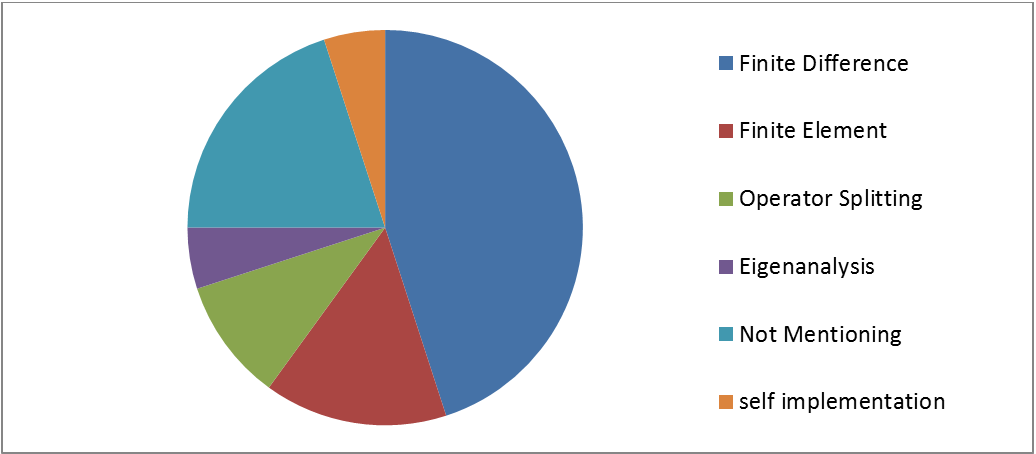
\includegraphics[totalheight=0.3\textheight,width=0.9\textwidth]{review_conclusion.png}
    \caption{Discretization Techniques}
    \label{fig:Conclusion Graph}
\end{figure}

Finally, an important conclusion about all the above papers concerns the methods that were most implemented for solving linear systems. In the following table, it is presented for each work the discretization method, the equation and the solver that was implemented. Most popular methods are Parallel Cyclic Reduction (PCR), Conjugate gradient (CG) and Jacobi. 

\begin{table}[t]
    \begin{center}
        \begin{tabular}{| l | p{4cm} | p{6cm} | p{6cm} |}
        \hline
        \#	& Discretization Method	& PDE equation 			 & Linear System Solver \\ \hline
        1	& Finite Difference	& 3D heat diffusion equation &	Jacobi \\ \hline
        2	& Finite Difference & 2D/3D Wave equation   	 &	- \\ \hline
        3	& Finite Difference	& 2D parabolic PDE	    	 & -  \\ \hline
        4	& -				    &	-						 & - \\ \hline
        5	&"naïve algorithm", "cached plane sweep", "pipelined wavefront" &	-	&- \\ \hline
        6	& Finite Difference	& the Cahn-Hilliard equation	& - \\ \hline
        7	& Finite Difference & the parabolic convection diffusion equation 	&Parallel cyclic reduction \\ \hline
        8	& Finite Difference	& focus on stochastic volatility models, the Hundsdorfer–Verwer scheme and the Douglas scheme	& ADI schemes \\ \hline
        9	& Eigenanalysis	& directional anisotropic diffusion \& coherence enhancing diffusion &	Explicit Euler scheme and an iterative method(self implemented) \\ \hline
        10	& Not Mentioning & -	& Hybrid tiled PCR \& p-Thomas  \\ \hline
        11	& Finite Element & The cardiac monodomain model (non linear ODE's and parabolic linear PDE's) &	2nd order Crank-Nikolson (PDE) \& explicit Euler (ODE)  \\ \hline
        12  & Finite Difference & the 2D wave equation \& the incompressible Navier-Stokes equations &	CG \& Gauss-Seidel\\ \hline
       13	& operator splitting	& Reaction diffusion equation	& Forward Euler \\ \hline
       14	& Finite Element and operator splitting	& the monodomain model	& Implicit and explicit solvers \\ \hline
        15	& - &	-	& SPIKE algorithm ,parallel diagonal pivoting \& p-Thomas\\ \hline
        16	& - &	Black-Scholes partial differential equation &	BiCGStab and CGS\\ \hline
        17	& Finite Difference	& OceanWave3D model 	& Iterative methods\\ \hline
        18	& - &	Helmholtz equation with Dirichlet and/or Neumann boundary conditions on the unit square &	CG and Multigrid  solvers\\ \hline
       19	& Finite Element	& Poisson problem on isotropic and anisotropic domains	& Multigrid, Jacobi, Gauss-Seidel, Thomas(CPU) and parallel Cyclic Reduction(GPU) \\ \hline
       20 &	- &	-	& CR,PCR,RD, Hybrid CR+PCR,CR+RD \\ \hline
       21	&  Finite Difference	& the parabolic convection diffusion equation &	Parallel cyclic reduction\\ \hline
        
        \hline
        \end{tabular}
    \end{center}

    \caption{Conclusion Table}
    \label{table:concl}
\end{table}



